% !TeX program = lualatex

\documentclass[british,a4paper]{article}

\usepackage{warnock}
\setmonofont{Hasklig}[Scale = MatchLowercase]
\usepackage{microtype}
\newfontfamily\tableroman{Warnock Pro}[Scale=MatchLowercase, Numbers={Monospaced,OldStyle}]

\usepackage{mVersion}
    \increaseBuild
    \setVersion{0.2}

\usepackage{csquotes}
\usepackage{babel}

\usepackage{geometry}
\usepackage{graphicx} 
\usepackage[export]{adjustbox} \usepackage{rotating} \usepackage{placeins}
\usepackage{fancyhdr}
    \pagestyle{fancy}
    \fancyhead{}\fancyfoot{}
    \fancyhead[R]{\version}
        \renewcommand{\headrulewidth}{0pt}
    \fancyfoot[C]{\thepage}

\usepackage{pdfpages}
\usepackage{lscape}

\usepackage{siunitx}
	\sisetup{detect-all, number-text-rm = \tableroman,output-decimal-marker = \text{.},table-alignment = center}
    \DeclareSIUnit{\annum}{a}
    \DeclareSIUnit{\years}{y}
    \DeclareSIPrefix\million{m}{6}
\usepackage[cleanlook]{isodate}

\usepackage{enumitem}

\setcounter{secnumdepth}{0}
\makeatletter 
    \renewcommand\listoffigures{%
	    \@starttoc{lof}%
    }
    \renewcommand\listoftables{%
	    \@starttoc{lot}%
    }
\makeatother

\usepackage{csvsimple}
\usepackage{tabu}
\usepackage{booktabs}
\usepackage{longtable}

\usepackage[style = nature, date = year]{biblatex}
    \addbibresource{biblio.bib}

\usepackage{hyperref}
\usepackage{cleveref}
    \newcommand\pcref[1]{(\cref{#1})}


\title{Supplemental material for ‘Early high rates and disparity in the evolution of fish-shaped reptiles’}
\author{Benjamin C.\ Moon \and Thomas L.\ Stubbs}
\date{\today~\version}

\begin{document}

\maketitle

\tableofcontents

\section{Supplemental methods}\label{supplemental-methods}

\paragraph{Comparison of time-scaling methods.}
\label{comparison-of-time-scaling-methods}

To assess the effects of variation in the timing of ichthyosaur evolution on discrete evolutionary rates, we further used the minimum branch length (MBL) tree-scaling method \autocite{Bapst2012, Laurin2004SystBiol}. This scales the tree according to occurrence dates, but ensures that each branch length is greater than a given value, rescaling ancestral branches as necessary to ensure this minimum length. Here, we used a MBL of \SI{1}{\mega\annum} as a reasonable minimum between speciation events and to avoid forcing excessive branch lengths where speciation may occur rapidly. We used the same sample of 120 phylogenetic trees as the main analysis from the Bayesian phylogenetic posterior distribution of \textcite{Moon2019a}. Trees were time-scaled in R \autocite{R} using the function \texttt{timePaleoPhy} in the package paleotree \autocite{Bapst2012} with point ages sampled from a uniform distribution between their first and last occurrences. Each tree was resampled 10 times to account for the occurrence ranges for each taxon (120 tree topologies × 10 samples = 1200 time-scaled trees total). These MBL time-scaled trees were then used for a further set of discrete character evolutionary rates analyses using function \texttt{DiscreteCharacterRate} of R package Claddis \autocite{Lloyd2016}. The results of this were used to produce `spaghetti' plots for epoch-length bins and equal-length bins using modified scripts from \textcite{Close2015a}. Code for all these analyses is included in Supplemental~\ref{disparity-discrete-code}.

\paragraph{Additional disparity metrics.}

Our main results present ichthyosauriform disparity using per-bin pairwise differences between taxa from a distance matrix calculated using maximum observed rescaled distances \autocite{Lloyd2016}. Additionally, we compared different distance conversion and disparity metrics.

Claddis provides four distance metrics for discrete character data \autocite{Lloyd2016}: raw Euclidean distances (RAW), generalized Euclidean distances (GED) \autocite{Wills1994}, Gower's coefficient (GOW) \autocite{Gower1971}, and maximum observable rescaled distances (MAX) \autocite{Lloyd2016}. All four distance metrics were run through the same disparity work flow. Recent studies have shown that GED as implemented in Claddis is susceptible to the completeness of the original data matrix, which may have a strong effect on the resulting disparity \autocite{Flannery-Sutherland2019, Lehmann2019}; therefore we prefer MAX.

Similarly, several different disparity metrics have been developed, each with varying properties. Our main results present mean and weighted mean pairwise distances on MAX as this comes directly from the original data matrix, but we also calculated the pairwise distances for RAW, GED, and GOW distances matrices \pcref{fig:pairwise-disparity}. We ordinated the data using Principal Coordinates Analysis (PCA), both with and without applying a correction to negative eigenvalues \autocite{Caillez1983} and compared the correlation of the PCA data with the original distance matrix. 

From the PCA data we used all the resultant axes to calculate per-bin sum of variances, sum of ranges, and centroid distances. These metrics have been used extensively in previous analyses \autocite{Wills1998, Thorne2011, Flannery-Sutherland2019}, so we considered it pertinent to compare them. Binning, bootstrap resampling with 10~000 replicates, and complete rarefaction were completed using the functions \texttt{custom.subsets} and \texttt{boot.matrix}, and disparity calculations used the function \texttt{dispRity}, all from package dispRity \autocite{Guillerme2018b} in R. Code for this is included in Supplemental~\ref{disparity-discrete-code}.


\section{Supplemental results}\label{sec:supplemental-results}

\paragraph{Pairwise disparity.}\label{par:pairwise-disparity}

Broadly speaking, trends in disparity across all four distance matrices are similar: disparity peaks in the Late Triassic then declines through the Jurassic and Cretaceous \pcref{fig:pairwise-disparity}. The bins that preserve the most completely coded taxa (\cref{fig:pairwise-disparity} CHAR: Early Jurassic; \SIrange{201.3}{171.3}{\mega\annum}) also show relatively increased disparity in RAW and GED distance matrices compared to GOW and MAX. Indeed, the earliest Jurassic bins are the most disparate for the RAW distance metric with both binning schemes, and for GED the earliest Jurassic bins have relatively higher disparity than GOW and MAX distance matrices. This is most likely a further effect of incompleteness degrading the disparity signal by averaging the difference between taxa \autocite{Flannery-Sutherland2019, Lehmann2019}, therefore we prefer the results given by GOW and MAX distance matrices.

\paragraph{Correlation of ordinated data.}\label{par:pco-correlation}

Negative eigenvalue correction notably decreased the variance described by the first few principal coordinate axes. The highest correlations between the original and ordinated data were found when including all ordinated axes \pcref{fig:ordination-correlation}. Without negative eigenvalue correction RAW and GED had the highest correlation, whereas GOW and MAX were reduced to \textasciitilde{}0.8. With negative eigenvalue correction the pattern of correlations with increasing number of axes was more complex: RAW gradually increased whereas GED strongly decreased, but both rapidly increased to 1.0 with the last axes; GOW and MAX correlations both immediately decreased, increased to a peak at \textasciitilde{}axis 60, then rapidly increased again when including the last axes.

\paragraph{Disparity of ordinated data.}\label{par:ordinated-disparity}

\textcite{Wills1998} asserted that variance based disparity metrics are more suited to measuring overall dissimilarity whereas range-based metrics are appropriate for disparity as they are affected by occurrence and thus show the diversification of morphology. In this context, our results support our conclusions that ichthyosaurs represent an early burst of evolution: both of these metrics show initial high disparity from all distance matrices (\cref{fig:ordinated-disparity}). Sum of variances also has a marked increase between the Early to Middle Triassic and a substantial decline in disparity between the Late Triassic–Early Jurassic in the combination of GOW/MAX distance matrix and uncorrected PCO; otherwise all curves follow similar t{}rends. Sum of variances proves more resilient to sample size in rarefaction than either sum of ranges or centroid distance (\cref{fig:rarefaction-curves}).

All sum of ranges curves display the same trends in disparity, differing only in the magnitude. Similarly, we find early high disparity and an increase between the Early–Middle Triassic (\cref{fig:ordinated-disparity}). Disparity decreases substantially through the later Triassic, but broadly recovers in the Early Jurassic before more log-term decline through to the extinction of the ichthyosaurs. Particularly low dis{}parity (e.g. Middle Jurassic; \SIrange{171.3} {161.3}{\mega\annum}) are those represented by few taxa and relative incompleteness.

In the case of centroid distance, although this has been shown to be especially susceptible to issues of centroid slippage' \autocite{Flannery-Sutherland2019, Lehmann2019}, our results show the same trends as for sum of variances: high early disparity that is sustained through to the Late Jurassic/Early Cretaceous before decline, with dips that are most likely related to incompleteness of specimens (\cref{fig:ordinated-disparity}).

\paragraph{Morphospace occupation of ordinated data.}\label{par:ordinated-morphospace}

Morphospace occupation between Triassic and post-Triassic Ichthyosauriformes is separated in almost all cases (\cref{fig:morphospace-plots}; except RAW and GED distances). Late Triassic taxa are also separated from earlier Triassic taxa in GOW and MAX distance without negative eigenvalue correction, and are consistently positioned more closely towards the Early Jurassic taxa. The variation in Jurassic and Cretaceous taxa is markedly increased in RAW and GED distances relative to GOW and MAX. Differences within Jurassic and Cretaceous taxa are more represented in PCo axis 2 than axis 3 in the RAW and GED morphospace plots, but in a combination of PCO axes 1 and 3 in GOW and MAX. All RAW and GED morphospace plots show more points towards the origins of the plots than GOW and MAX, a results of 'centroid slippage' \autocite{Flannery-Sutherland2019, Lehmann2019}; in particular these represent the least complete taxa.

\paragraph{Time-scaling and rates.}\label{par:mbl-scaling-rates}

Using the MBL time-scaling method created trees with a root age of \SIrange{253.8}{268.5}{\mega\annum}; older than the corresponding root ages from the Hedman scaling method. Rates of discrete character evolution are relatively lower for during the Early–Middle Triassic, but these earlier bins nonetheless show significantly higher rates of evolution that subsequent bins \pcref{fig:mbl-discrete-rates}. Trends across the whole of ichthyosaur evolution remain similar, although there are increased peaks in the later Early Jurassic and the Late Cretaceous bins. Significantly low rates of discrete character evolution are reached in the Early Jurassic (epoch bins) or Late Triassic (\SI{10}{\mega\annum} bins).



\section{Supplemental figures}\label{sec:supplemental-figures}

\listoffigures

\begin{figure}[h]
    % 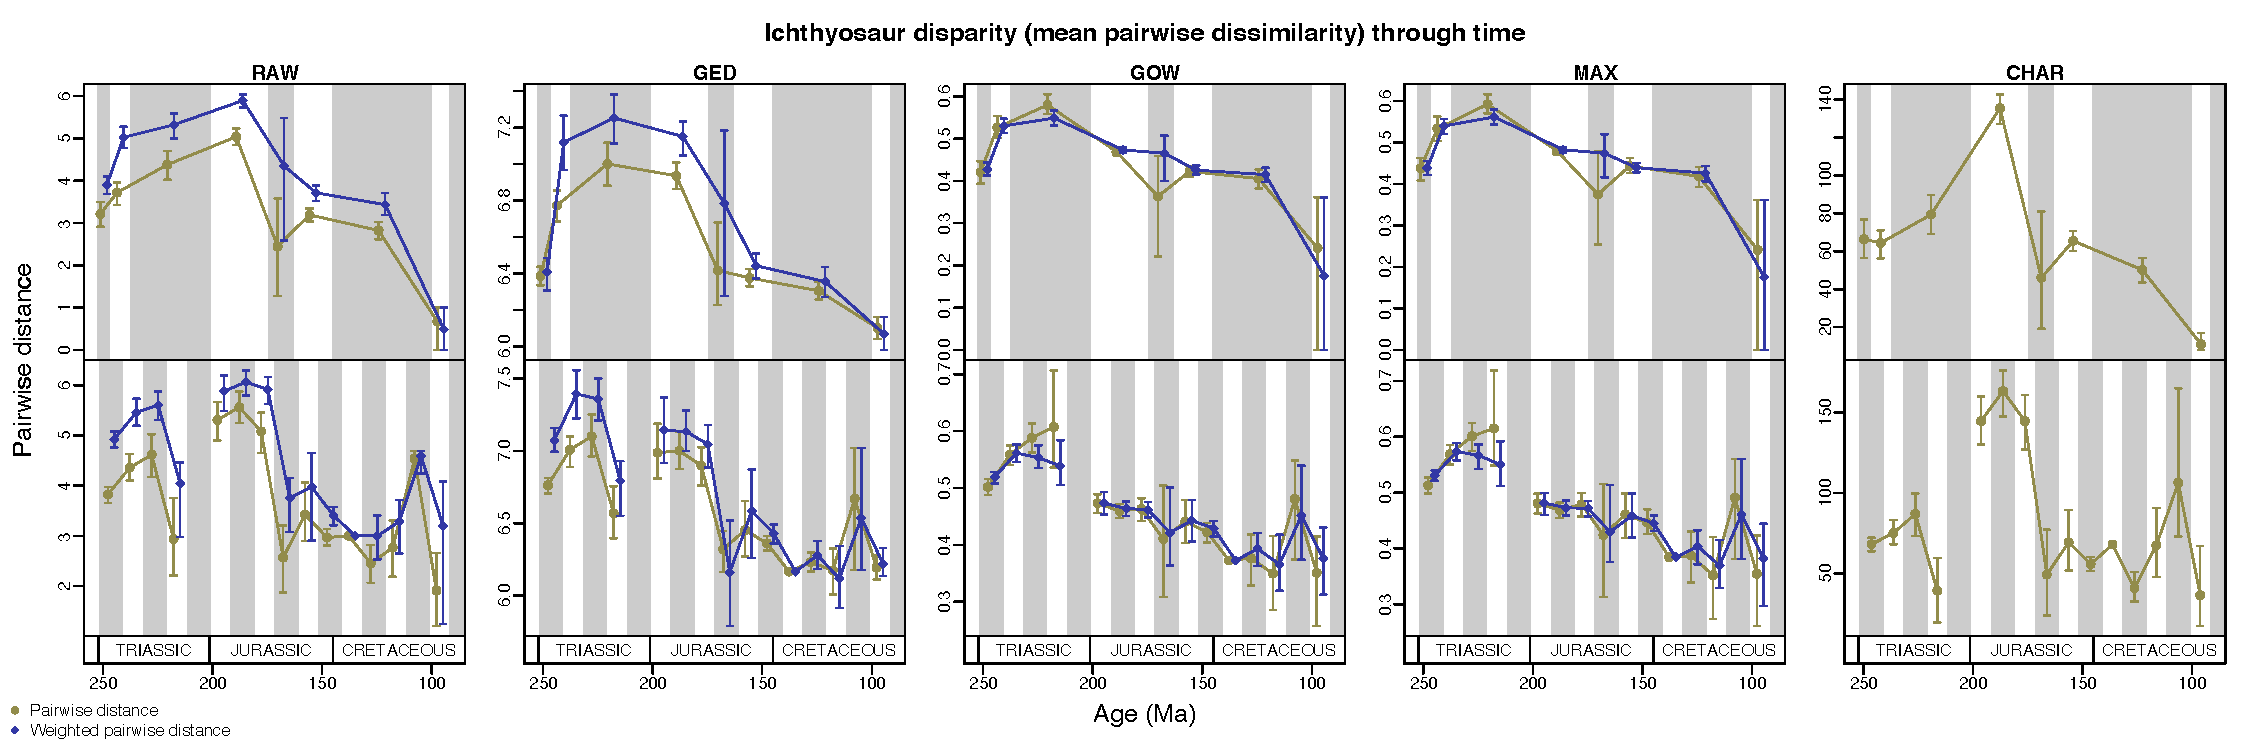
\includegraphics[width = \textheight, center]{supp_figures/figS3-pairwise_all}
    \caption[Per-bin discrete skeletal disparity of Ichthyosauriformes though the Mesozoic]{(following page) \textbf{Per-bin discrete skeletal disparity of Ichthyosauriformes though the Mesozoic.} Pairwise and weighted pairwise dissimilarity measured from raw Euclidean (RAW), generalised Euclidean (GED), Gower (GOW), and maximum observed rescaled (MAX) distances between taxa in the cladistic dataset of \textcite{Moon2019a} binned into epochs and equal 10-million-year bins. Also, pairwise number of comparable characters between taxa (CHAR) indicating the variation in completeness and comparability in each bin. Mean values and 95\% confidence intervals are shown from 10,000 bootstrap replicates.\label{fig:pairwise-disparity}} 
\end{figure} \FloatBarrier

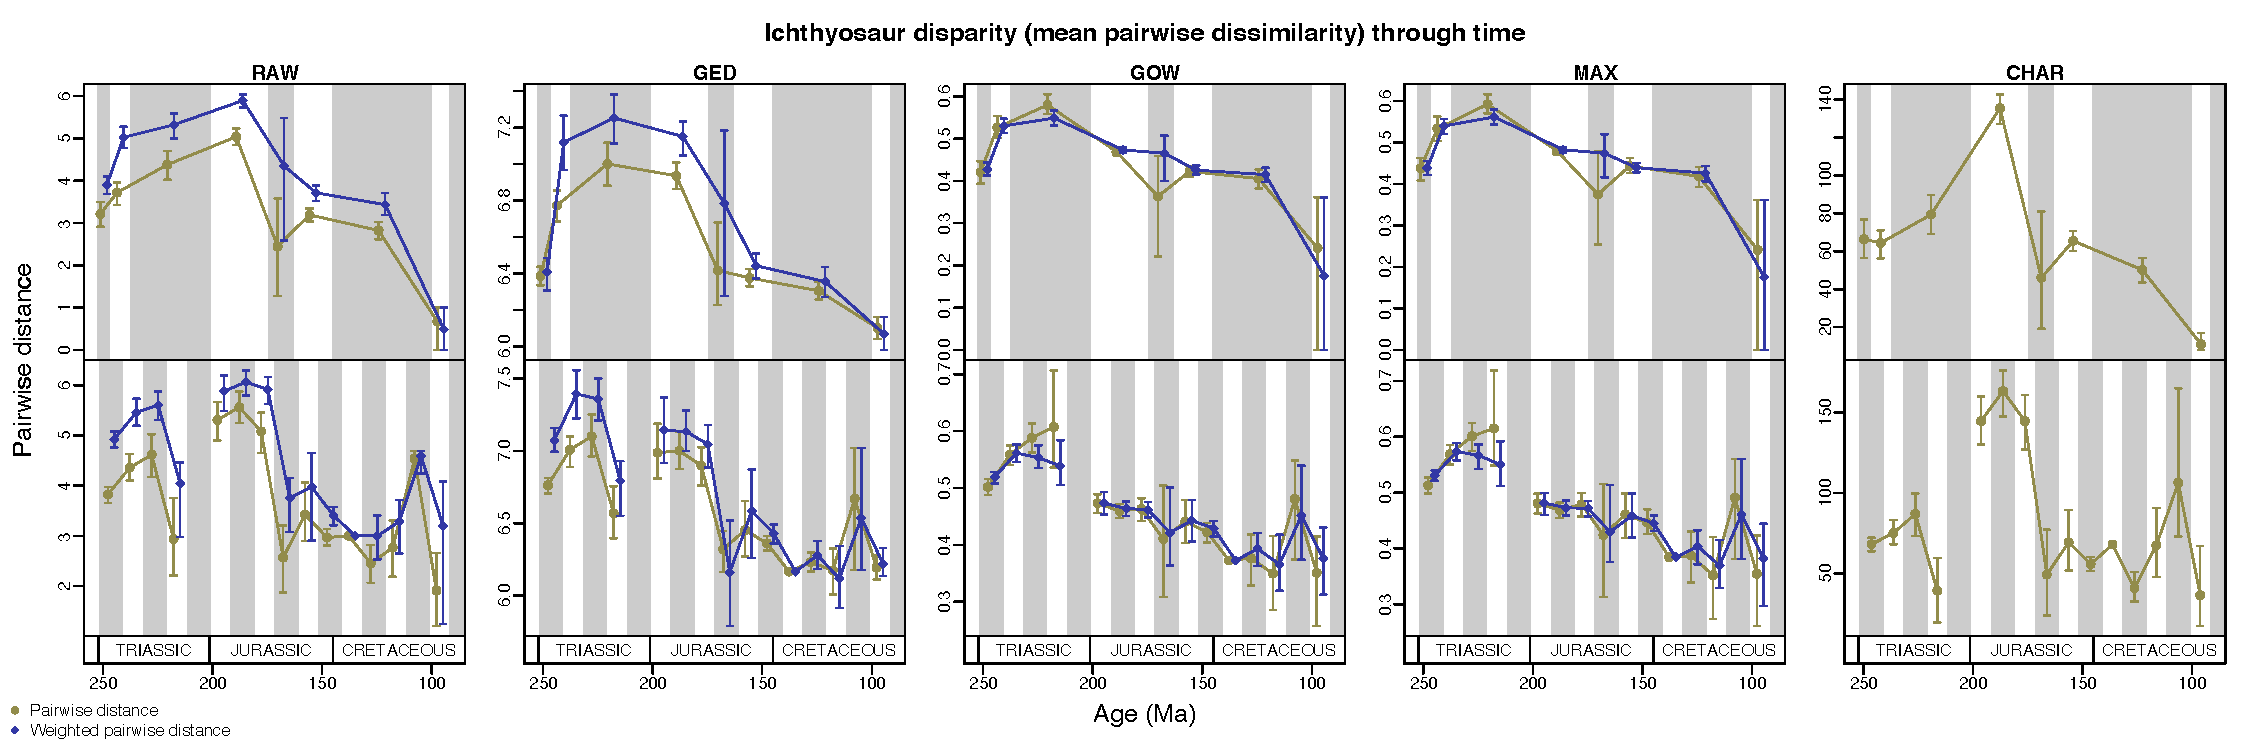
\includepdf[pages = -, fitpaper = true]{supp_figures/figS3-pairwise_all.pdf}
\FloatBarrier

\begin{figure}[h]
    \caption[Per-bin discrete skeletal disparity of Ichthyosauriformes through the Mesozoic from ordinated data]{(following pages) \textbf{Per-bin discrete skeletal disparity of Ichthyosauriformes through the Mesozoic from ordinated data.} Ichthyosaur disparity represented by mean sum of variances, mean sum of ranges, and mean centroid distance from each of eight PCA (four distance matrices: RAW, GED, GOW, MAX; with and without negative eigenvalue correction) on the cladistic matrix of \textcite{Moon2019a}. Error bars show 95\% confidence intervals from 10,000 bootstrap replicates.\label{fig:ordinated-disparity}}
\end{figure}
\FloatBarrier

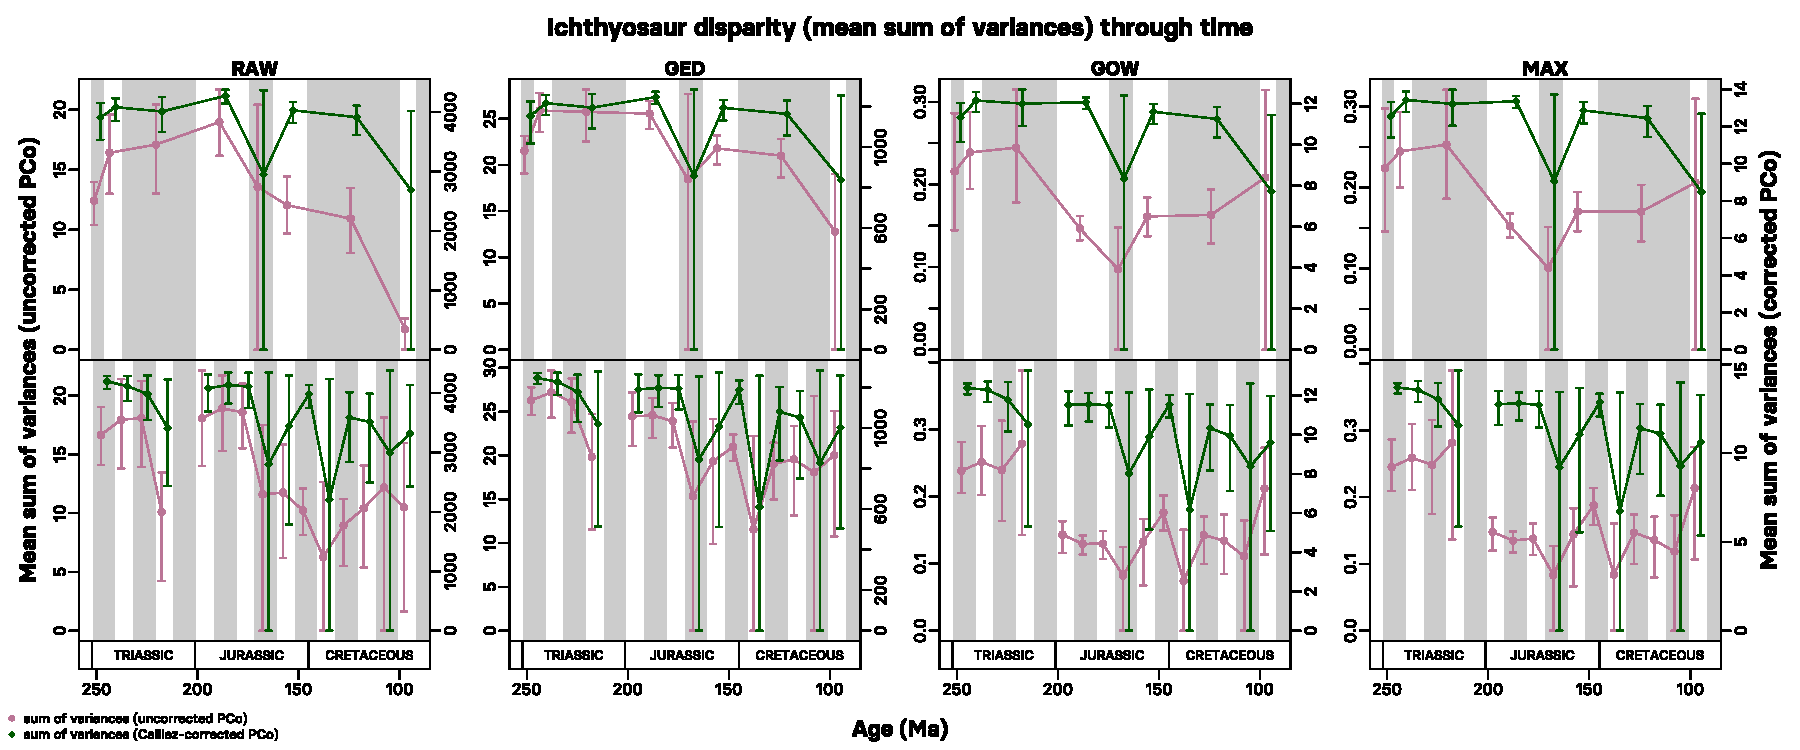
\includepdf[pages=-, fitpaper = true]{supp_figures/figS5-disparity_time.pdf}
\FloatBarrier

\begin{figure}[h]
    \caption[Per-bin rarefaction curves for each disparity-time curve shown in \cref{fig:ordinated-disparity}]{(following pages) \textbf{Per-bin rarefaction curves for each disparity-time curve shown in \cref{fig:ordinated-disparity}} Disparity for each bin is sequentially rarefied on taxon occurrences. Error polygon gives 95\% confidence interval from 10,000 bootstrap replicates.\label{fig:rarefaction-curves}}
\end{figure}
\FloatBarrier

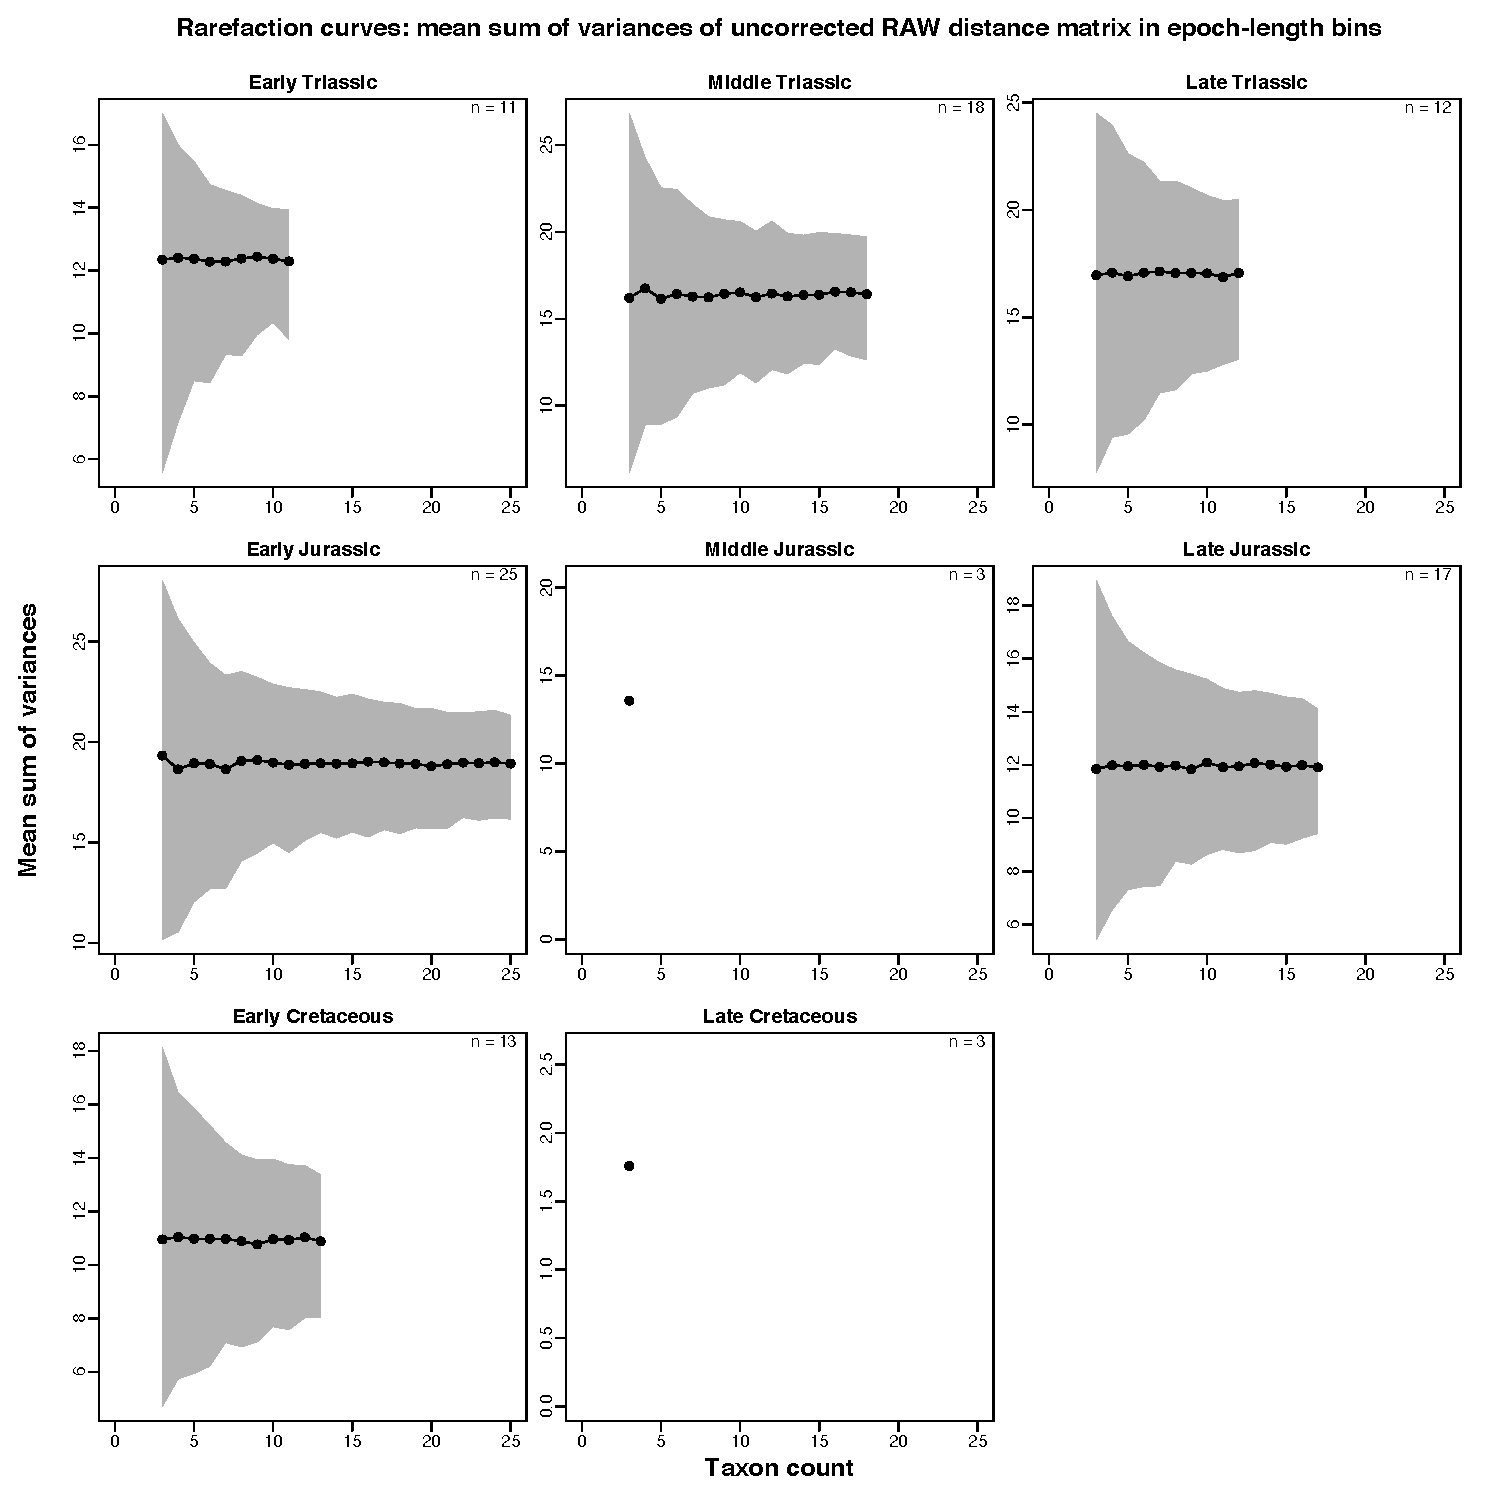
\includepdf[pages = -, fitpaper = true]{supp_figures/figS6-rarefaction_curves.pdf}
\FloatBarrier

\begin{figure}[h]
    \caption[Morphospace occupation of Ichthyosauriformes through the Mesozoic]{(following pages) \textbf{Morphospace occupation of Ichthyosauriformes through the Mesozoic.} Principal coordinate axis 1 against axes 2 (top row) and 3 (bottom row) from each of eight PCA (four distance matrices: RAW, GED, GOW, MAX; with and without negative eigenvalue correction) on the cladistic matrix of \textcite{Moon2019a} binned into epochs.\label{fig:morphospace-plots}}
\end{figure}
\FloatBarrier

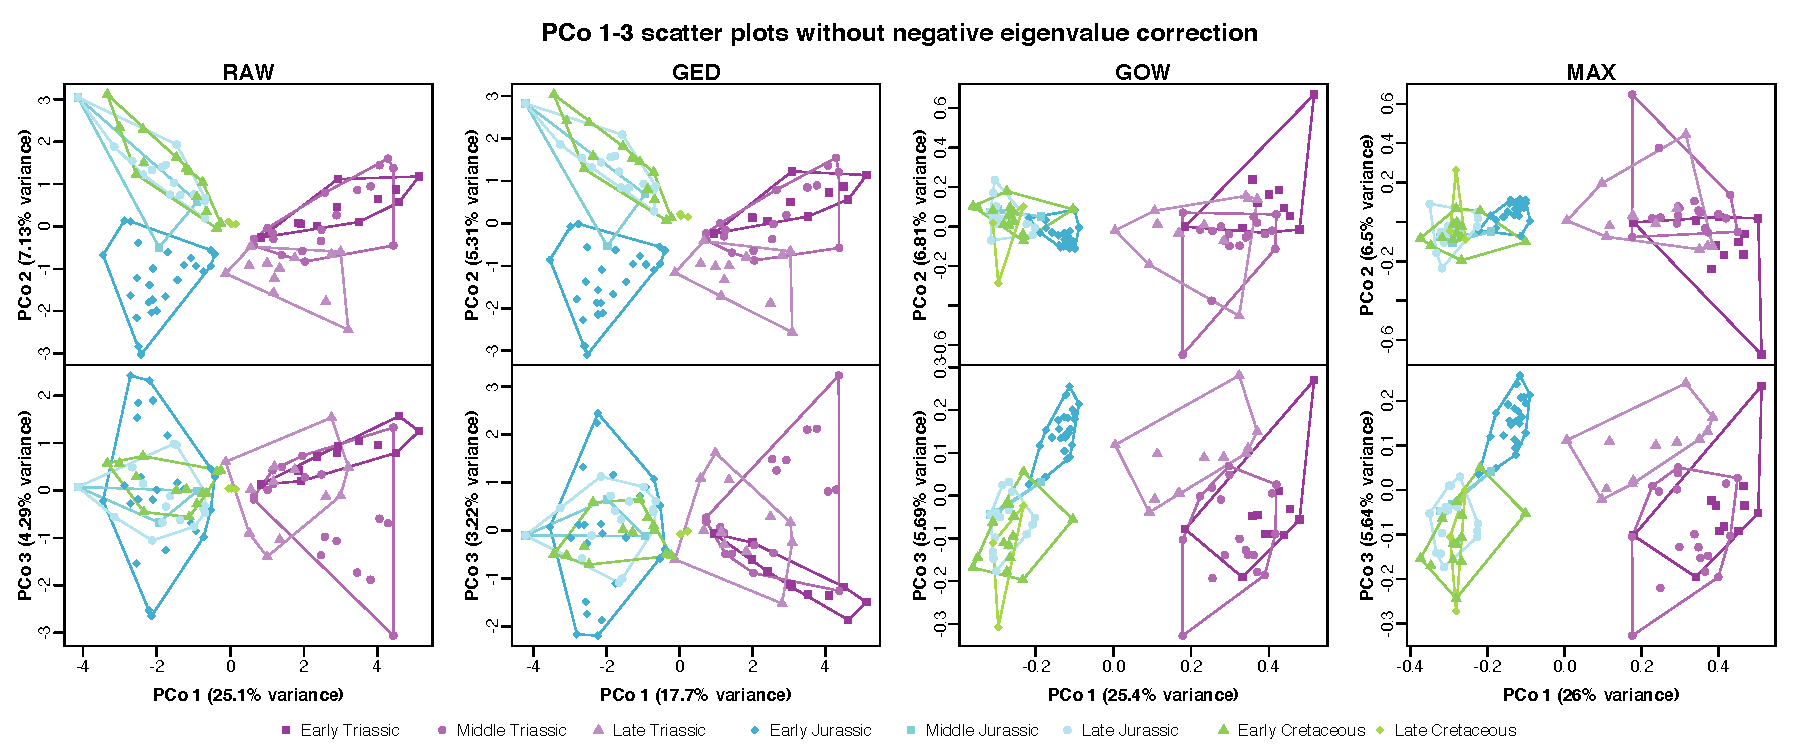
\includepdf[pages = -, fitpaper = true]{supp_figures/figS7-all_morphospace.pdf}


\begin{figure}[h]
    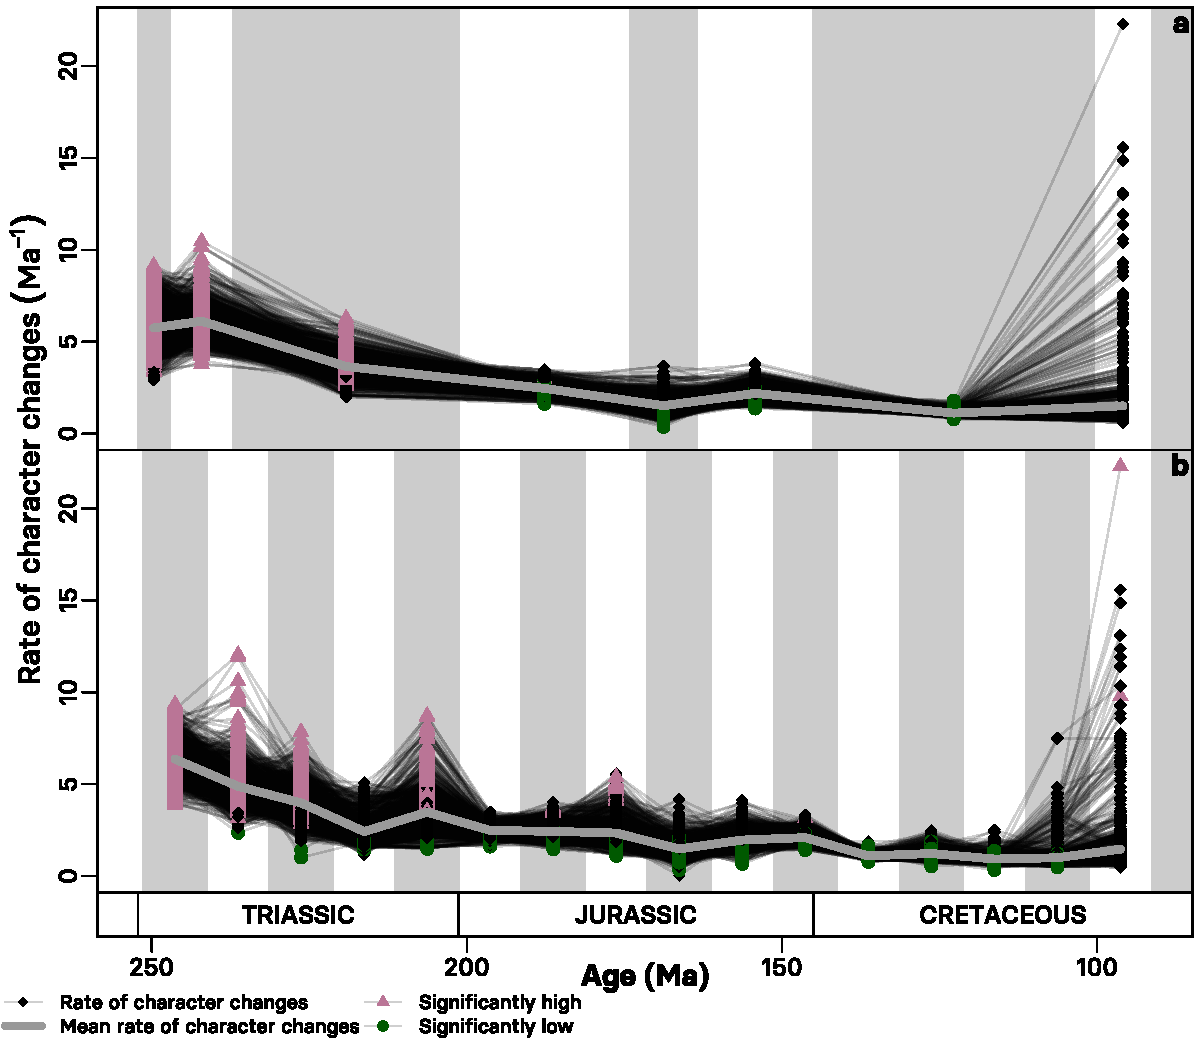
\includegraphics[width = \textwidth, center]{supp_figures/figS8-rates_MBLspaghetti}
    \caption[Rates of discrete skeletal character evolution in Ichthyosauriformes]{\textbf{Rates of discrete skeletal character evolution in Ichthyosauriformes.} Calculated from the matrix of \textcite{Moon2019a} using 1200 time-scaled trees from the minimum branch length method. Rates of evolution are plotted in \textbf{a}, epoch-bins and \textbf{b}, equal-length 10-million-year bins. \label{fig:mbl-discrete-rates}} 
\end{figure}
\FloatBarrier
 
\begin{figure}
\caption[Rates of skull size evolution in Ichthyosauriformes]{(following
	page) \textbf{Rates of skull size evolution in Ichthyosauriformes.}
	Evolutionary rate results from 100 Hedman-dated phylogenies. Branches
	are scaled and branches and taxon names coloured to the rate of skull
	size change on that branch.} 
\end{figure} 
\FloatBarrier

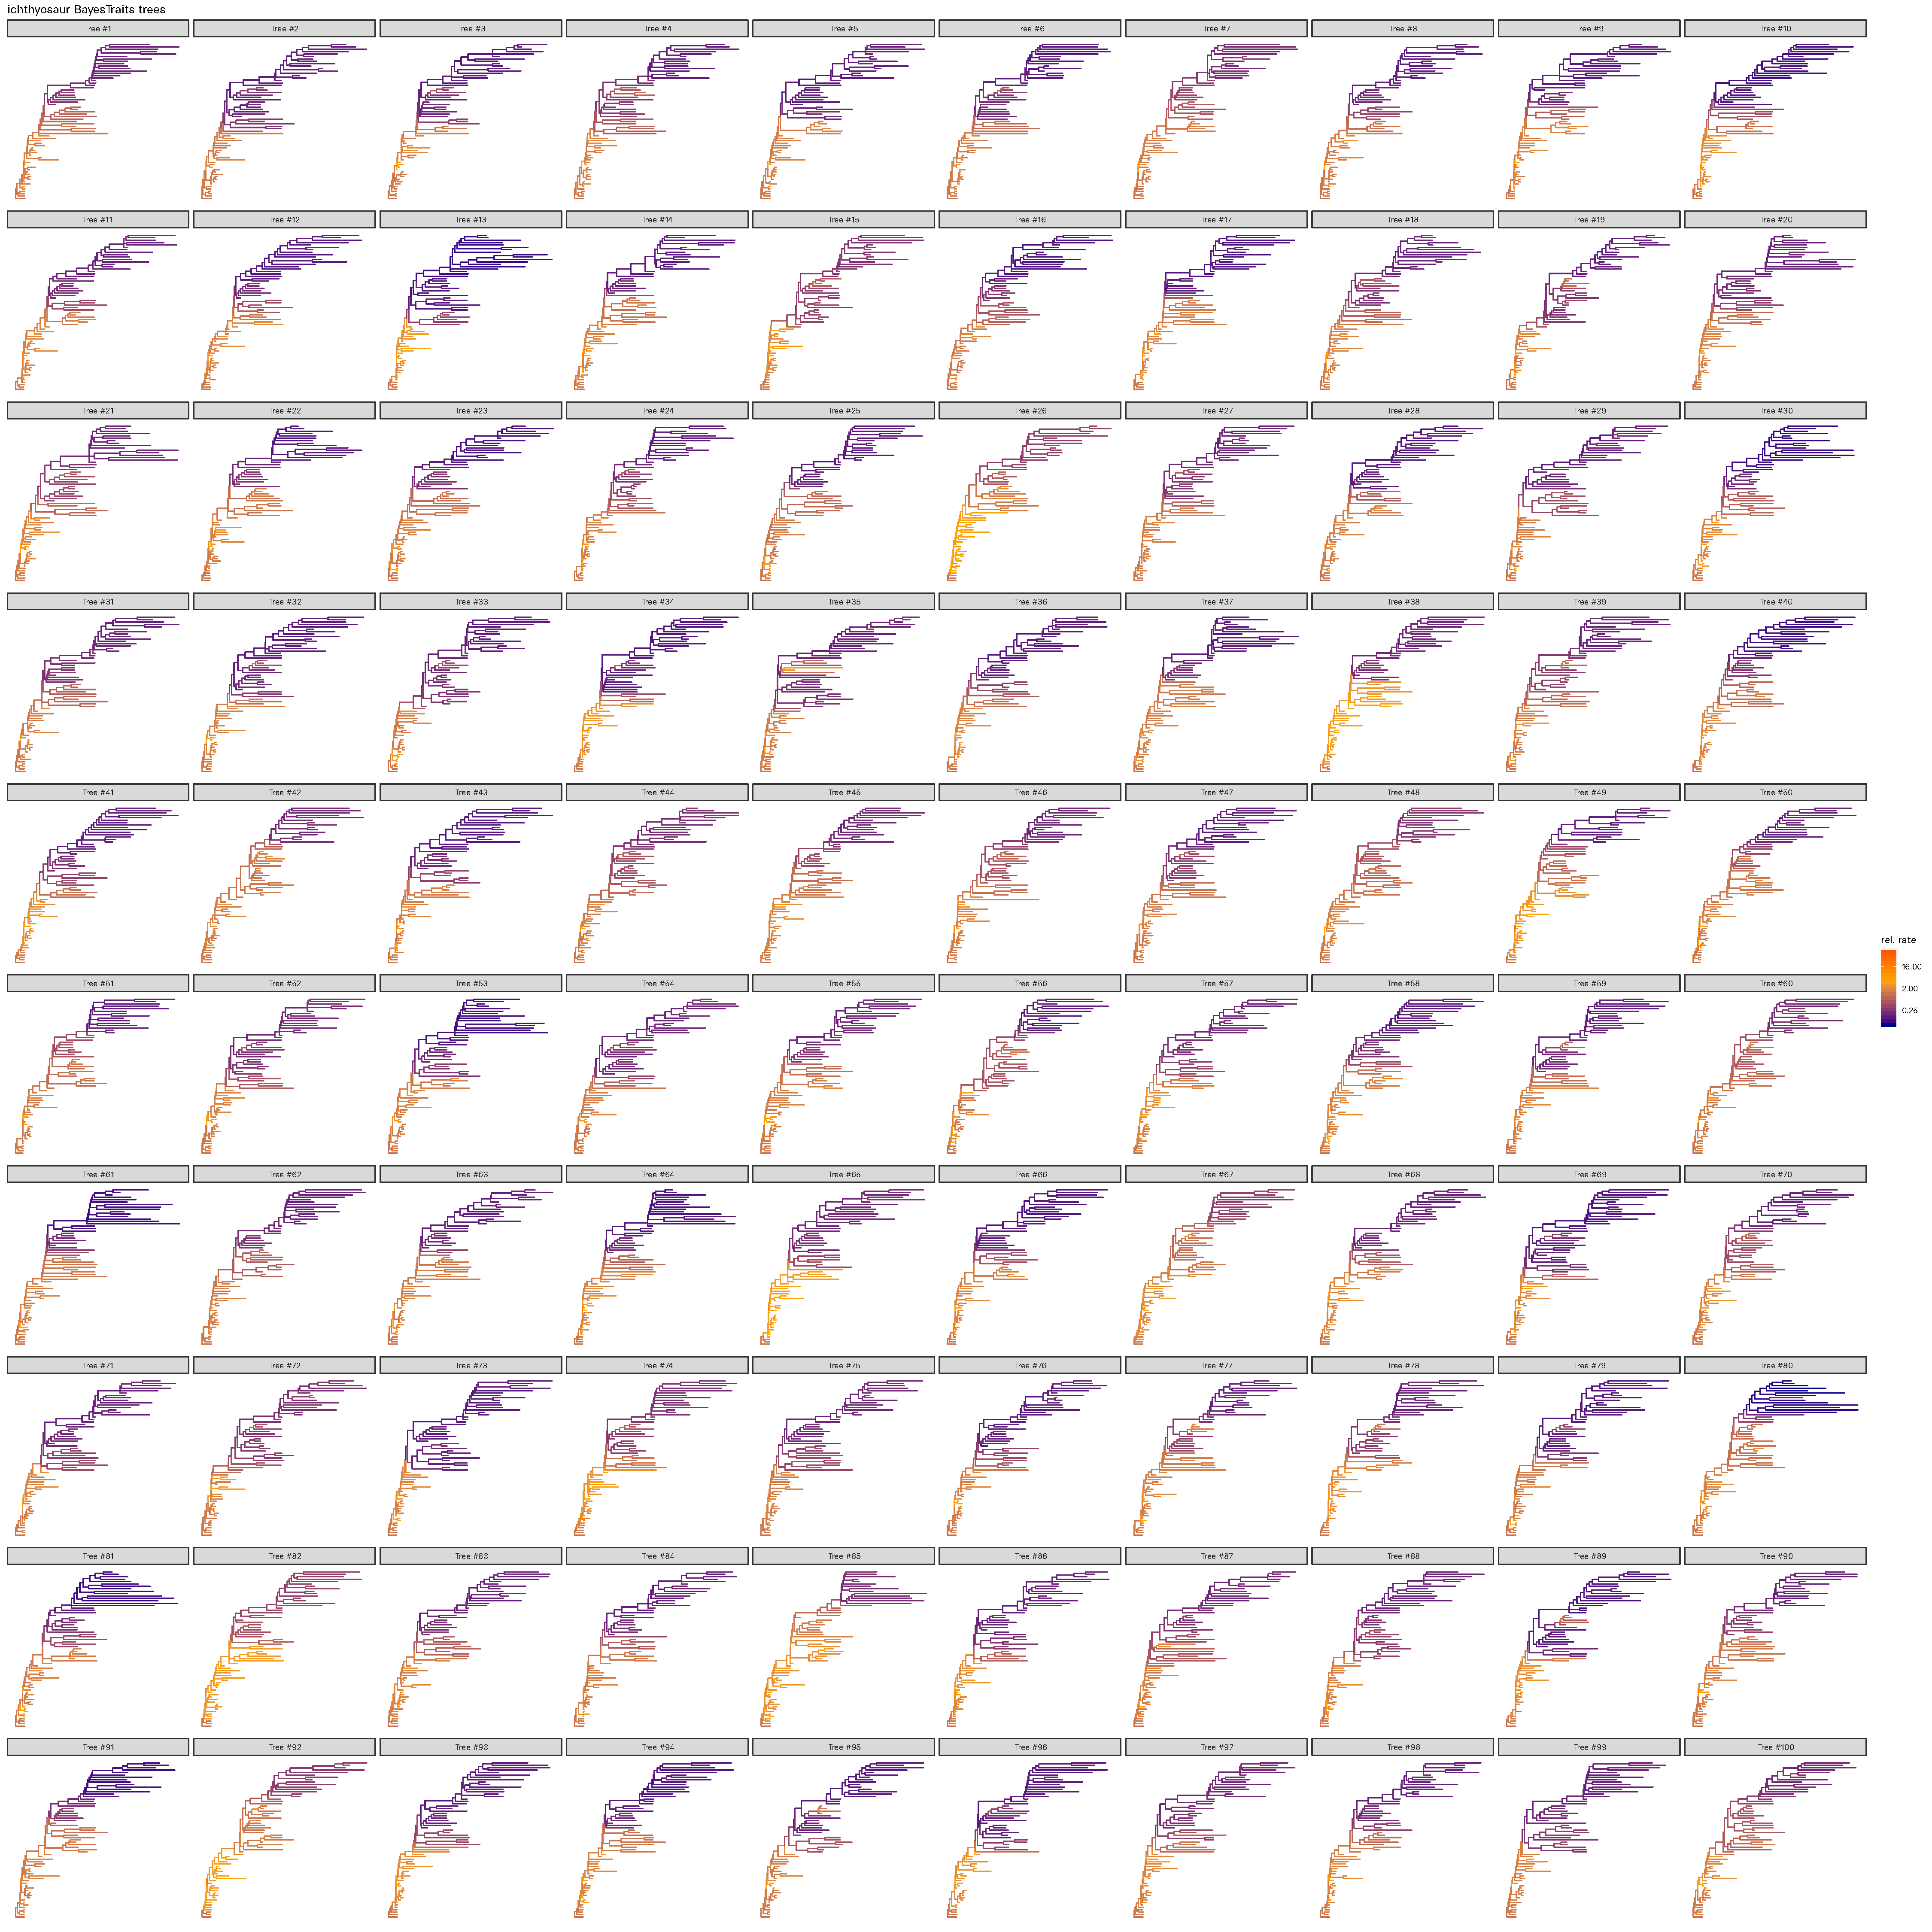
\includepdf[pages = -, fitpaper = true]{supp_figures/figS10-bayestraits_trees_rates.pdf}

\restoregeometry

\section{Supplementary tables}\label{supplementary-tables}

\listoftables

\begin{table}[h]
	\caption[Bin boundaries of \SI{10}{\mega\annum} bins used in this study]{\textbf{Bin boundaries of \SI{10}{\mega\annum} bins used in this study.} Approximate age ranges are given as indicators.\label{tbl:ten-ma-bins}}
	\csvreader[%
		centered tabular = rSSl,
		table head = {\toprule {Bin} & {Start (\si{\mega\annum})} & {End (\si{\mega\annum})} & {Approximate age range} \\\midrule},
		table foot = \bottomrule]%
		{supp_tables/10ma-dates.csv}%
		{}%
		{\csvlinetotablerow}
\end{table}

\begin{table}[h]
    \caption[Occurrence dates of outgroup taxa used to date the tree of Ichthyosauriformes]{\textbf{Occurrence dates of outgroup taxa used to date the tree of Ichthyosauriformes.} Stratigraphic occurrence intervals are taken from the given references. Occurrences are converted to absolute ages using \textcite{Gradstein2012}. FAD, first appearance date; FAS, first appearance stratigraphy; LAD, last appearance date; LAS, last appearance stratigraphy.\label{tbl:outgroup-dates}}
    \small
    \csvreader[%
	    tabular = >{\itshape}lSSlll,
	    table head = \toprule \emph{Taxon} & {FAD (\si{\mega\annum})} & {LAD (\si{\mega\annum})} & FAS & LAS & Reference\\\midrule,
        late after last line = \\\bottomrule]%
        {supp_tables/outgroup_dates.csv}%
        {Taxon=\taxon,FAD=\fad,LAD=\lad,FAStrat=\fas,LAStrat=\las,Reference=\ref}%
        {\taxon & \fad & \lad & \fas & \las & \ref}
\end{table}

\begin{landscape}
	{\footnotesize%\defaultfontfeatures+{Numbers = {OldStyle,Monospaced}}
		%! TEX root = ../supplement-ichthyosaur_macroevolution.tex
%! BIB file = zotero.bib

\begin{longtabu}{>{\itshape}lXXSSl}
	\caption[Occurrence stratigraphy and dates of Ichthyosauriformes included in the analyses]{{\normalsize\textbf{Occurrence stratigraphy and dates of Ichthyosauriformes included in the analyses.} Stratographical occurrences are given to the nearest ammonite or conodont biozone horizon where possible. Occurrences are converted to absolute ages using \textcite{Gradstein2012}. FAD, first appearance date; LAD, last appearance date.\label{tbl:ingroup-dates}}}\\                                                      
	\toprule\emph{Taxon}                                 & {FAD stratigraphy}                                                                                                                 & {LAD stratigraphy}                                                                                                                 & {FAD (\si{\mega\annum})} & {LAD (\si{\mega\annum})} & {References} \\\midrule\endfirsthead     
	\caption*{Table~\thetable{} continued}\\
	\toprule\emph{Taxon}                                 & {FAD stratigraphy}                                                                                                                 & {LAD stratigraphy}                                                                                                                 & {FAD (\si{\mega\annum})} & {LAD (\si{\mega\annum})} & {References} \\\midrule\endhead          
	\bottomrule\endfoot
	\bottomrule\endlastfoot
	Acamptonectes densus                                 & \textallsc{D2D}
        horizon, Speeton Clay Formation, basal Hauterivian
                                                             & \emph{Simbiskites
    concinnus/staffi} Biozone, upper Hauterivian, Lower Cretaceous
                                                             & 132.9
                                                             & 129.4
                                                             &
                                                             \cite{Fischer2012PO} \\                   
	Aegirosaurus leptospondylus                          & Malm Zeta2b,
        early lower Tithonian, Upper Jurassic
                                                             & Malm Zeta2b,
        early lower Tithonian, Upper Jurassic
                                                             & 153.96
                                                             & 149.87
                                                             &
                                                             \cite{Bardet2000JP} \\                     
	Arthropterygius chrisorum                            & Oxfordian, Upper
        Jurassic
                                                             & Kimmeridgian,
        Upper Jurassic
                                                             & 163.47
                                                             & 152.06
                                                             &
                                                             \cite{Maxwell2010JVP} \\                    
	Athabascasaurus bitumineus                           & Lower Albian,
        Lower Cretaceous
                                                             & Lower Albian,
        Lower Cretaceous
                                                             & 113
                                                             & 111.5
                                                             &
                                                             \cite{Druckenmiller2010CJES} \\              
	Barracudasauroides panxianensis                      & \emph{Nicoraella
        germanicus} Conodont Biozone, Anisian, Middle Triassic
                                                             & \emph{Nicoraella
        germanicus} Conodont Biozone, Anisian, Middle Triassic
                                                             & 244.94
                                                             & 243.99
                                                             &
                                                             \cite{Jiang2006JVP} \\                      
	Besanosaurus leptorhynchus                           & \emph{Nevadites}
        Conodont Biozone, uppermost Anisian, Middle Triassic
                                                             & \emph{Nevadites}
        Conodont Biozone, uppermost Anisian, Middle Triassic
                                                             & 242.1
                                                             & 241.5
                                                             &
                                                             \cite{DalSasso1996PL} \\                   
	Brachypterygius extremus                             &
        \emph{Pectinatites wheatleyensis} Ammonite Biozone, Tithonian, Upper
        Jurassic                                                      &
        \emph{Pectinatites hudlestoni} Ammonite Biozone, Tithonian, Upper
        Jurassic                                                         & 151
                                                                         & 150
                                                                         &
                                                                         \cite{Moon2018MPS} \\                       
	Brachypterygius pseudoscythica                       & \emph{Ilowaisya
        pseudoscythica} Ammonite Biozone, Tithonian, Upper Jurassic
                                                             & \emph{Ilowaisya
        pseudoscythica} Ammonite Biozone, Tithonian, Upper Jurassic
                                                             & 150.1
                                                             & 149.5
                                                             &
                                                             \cite{Efimov1998PZ} \\                     
	Californosaurus perrini                              &
        \emph{Trachyceras} Beds, Hosselkus Limestone, Carnian
                                                             &
        \emph{Trachyceras} Beds, Hosselkus Limestone, Carnian
                                                             & 233.5
                                                             & 228.35
                                                             &
                                                             \cite{Merriam1902UCBDG,Merriam1908MUC} \\        
	Callawayia neoscapularis                             &
        \emph{Epigondolella triangularis} Conodont Biozone, early Norian, Upper
        Triassic                                                   &
        \emph{Epigondolella quadrata} Conodont Biozone, early Norian, Upper
        Triassic                                                       & 221.5
                                                                       & 217.5
                                                                       &
                                                                       \cite{McGowan1994JVPa} \\                   
	Cartorhynchus lenticarpus                            &
        \emph{Subcolumbites} Ammonite Biozone, Olenekian, Lower Triassic
                                                             &
        \emph{Subcolumbites} Ammonite Biozone, Olenekian, Lower Triassic
                                                             & 247.7
                                                             & 247.2
                                                             &
                                                             \cite{Motani2015N} \\                    
	Caypullisaurus bonapartei                            &
        \emph{Virgatosphinactes mendozanus} Ammonite Biozone, early Tithonian,
        Upper Jurassic                                              & Berriasian
                                                                    & 152.1
                                                                    & 139.4
                                                                    &
                                                                    \cite{Fernandez1997JP} \\                 
	Chacaicosaurus cayi                                  & \emph{Emileia
        giebeli} Ammonite Biozone, early Bajocian, Middle Jurassic
                                                             & \emph{Emileia
        giebeli} Ammonite Biozone, early Bajocian, Middle Jurassic
                                                             & 170.3
                                                             & 169.45
                                                             &
                                                             \cite{Fernandez1994A} \\                  
	Chaohusaurus chaoxianensis                           &
        \emph{Procolumbites} Ammonite Biozone, Olenekian, Lower Triassic
                                                             &
        \emph{Subcolumbites} Ammonite Biozone, Olenekian, Lower Triassic
                                                             & 247.9
                                                             & 247.2
                                                             &
                                                             \cite{Motani2014PO,Motani2015JVP} \\          
	Chaohusaurus geishanensis                            &
        \emph{Procolumbites} Ammonite Biozone, Olenekian, Lower Triassic
                                                             &
        \emph{Subcolumbites} Ammonite Biozone, Olenekian, Lower Triassic
                                                             & 247.9
                                                             & 247.2
                                                             &
                                                             \cite{Motani2014PO,Motani2015JVP} \\         
	Chaohusaurus zhangjiawanensis                        &
        \emph{Neospathodus homeri} Conodont Biozone, Spathian, Lower Triassic
                                                             &
        \emph{Neospathodus triangulus} Conodont Biozone, Spathian, Lower
        Triassic                                                          &
        247.9                    & 247.2                    & \cite{Chen2013AGS} \\                       
	Contectopalatus atavus                               & Pelsonian,
        Anisian, Middle Triassic
                                                             & Illyrian,
        Anisian, Middle Triassic
                                                             & 244.94
                                                             & 241.5
                                                             & \cite{Liu2013P} \\                        
	Cryopterygius kielanae                               & Middle Volgian,
        Lower Tithonian, Upper Jurassic
                                                             & Middle Volgian,
        Lower Tithonian, Upper Jurassic
                                                             & 149
                                                             & 147
                                                             &
                                                             \cite{Tyborowski2016APP} \\                 
	Cryopterygius kristiansenae                          &
        \emph{Dorsoplanites maximus} Ammonite biozone, Tithonian, Upper Jurassic
                                                             &
        \emph{Dorsoplanites ilovaiskyi} Ammonite biozone, Tithonian, Upper
        Jurassic                                                        & 148.3
                                                                        & 147.4
                                                                        &
                                                                        \cite{Druckenmiller2012NJG} \\             
	Cymbospondylus buchseri                              & Upper Anisian,
        Middle Triassic
                                                             & lower Ladinian,
        Middle Triassic
                                                             & 242.57
                                                             & 240.3
                                                             &
                                                             \cite{Sander1989JVP} \\                     
	Cymbospondylus nichollsi                             & \emph{Kellnerites
        felsoeoersensis} Ammonite Biozone, Anisian, Middle Triassic
                                                             & \emph{Kellnerites
        felsoeoersensis} Ammonite Biozone, Anisian, Middle Triassic
                                                             & 243.99
                                                             & 243.05
                                                             &
                                                             \cite{Frobisch2006ZJLS} \\                   
	Cymbospondylus petrinus                              &
        \emph{Paragondolella} ex gr. \emph{excelsa} Conodont Biozone, Anisian,
        Middle Triassic                                             &
        \emph{Paragondolella} ex gr. \emph{excelsa} Conodont Biozone, Anisian,
        Middle Triassic                                             & 243.99
                                                                    & 241.5
                                                                    &
                                                                    \cite{Merriam1908MUC} \\                    
	Cymbospondylus piscosus                              & Anisian, Middle
        Triassic
                                                             & Anisian, Middle
        Triassic
                                                             & 247.2
                                                             & 241.5
                                                             &
                                                             \cite{Merriam1908MUC} \\                    
	Dearcmhara schawcrossi                               & \emph{Pleydellia
        aalensis} Ammonite Biozone, Toarcian, Lower Jurassic
                                                             &
            \emph{Stephanoceras humphriesianum} Ammonite Biozone, Bajocian,
            Middle Jurassic                                                    &
            174.43                   & 169.45                   &
            \cite{Brusatte2015SJG} \\                   
	Eurhinosaurus longirostris                           &
        \emph{Dactylioceras tenuicostatum} Ammonite Biozone, Toarcian
                                                             & \emph{Harpoceras
    falciferum} Ammonite Biozone, Toarcian
                                                             & 182.7
                                                             & 180.36
                                                             &
                                                             \cite{vonHuene1951NJGPA,McGowan1986N} \\          
	Excalibosaurus costini                               & \emph{Arietites
        bucklandi} Ammonite Biozone, lower Sinemurian, Lower Jurassic
                                                             & \emph{Arietites
        bucklandi} Ammonite Biozone, lower Sinemurian, Lower Jurassic
                                                             & 199.3
                                                             & 197.8
                                                             &
                                                             \cite{McGowan2003JVP,McGowan1986N} \\        
	Gengasaurus nicosiai                                 & Calcari ad aptici
        e Saccocoma Formation, Late Kimmeridgian, Upper Jurassic
                                                             & earliest
        Tithonian, Upper Jurassic
                                                             & 155
                                                             & 150
                                                             &
                                                             \cite{Paparella2016GM} \\                  
	Grendelius alekseevi                                 &
        \emph{Dorsoplanites panderi} Ammonite Biozone, Tithonian, Upper Jurassic
                                                             &
        \emph{Dorsoplanites panderi} Ammonite Biozone, Tithonian, Upper Jurassic
                                                             & 149.6
                                                             & 147.9
                                                             &
                                                             \cite{Arkhangelsky2001PJ} \\               
	Grendelius zhuravlevi                                & Middle Volgian,
        Lower Tithonian, Upper Jurassic
                                                             & Middle Volgian,
        Lower Tithonian, Upper Jurassic
                                                             & 149.6
                                                             & 147.9
                                                             &
                                                             \cite{Zverkov2015PZIRa} \\                   
	Grippia longirostris                                 &
        \emph{Subcolumbites} Ammonite Biozone, Olenekian, Lower Triassic
                                                             &
        \emph{Subcolumbites} Ammonite Biozone, Olenekian, Lower Triassic
                                                             & 247.7
                                                             & 247.2
                                                             & \cite{Motani2000P} \\                     
	Guizhouichthyosaurus tangae                          & Carnian, Upper
        Triassic
                                                             & Carnian, Upper
        Triassic
                                                             & 233.5
                                                             & 228.35
                                                             &
                                                             \cite{Pan2006ASNUP} \\                        
	Guizhouichthyosaurus wolonggangense                  & Carnian, Upper
        Triassic
                                                             & Carnian, Upper
        Triassic
                                                             & 233.5
                                                             & 228.35
                                                             & \cite{Chen2007GC} \\                       
	Gulosaurus helmi                                     &
        \emph{Subcolumbites} Ammonite Biozone, Olenekian, Lower Triassic
                                                             &
        \emph{Subcolumbites} Ammonite Biozone, Olenekian, Lower Triassic
                                                             & 247.7
                                                             & 247.2
                                                             &
                                                             \cite{Brinkman1992P,Cuthbertson2013JVP} \\  
	Hauffiopteryx typicus                                &
        \emph{Dactylioceras tenuicostatum}, Ammonite Biozone, Toarcian
                                                             & \emph{Harpoceras
    falciferum} Ammonite Biozone, Toarcian
                                                             & 182.7
                                                             & 181.25
                                                             &
                                                             \cite{Maisch2008P,Caine2011P,Marek2015P} \\
	Himalayasaurus tibetensis                            & Norian, Upper
        Triassic
                                                             & Norian, Upper
        Triassic
                                                             & 228.4
                                                             & 209.5
                                                             & \cite{Motani1999P} \\                    
	Hudsonelpidia brevirostris                           &
        \emph{Epigondolella quadrata} Conodont Biozone, Norian, Upper Triassic
                                                             &
        \emph{Epigondolella quadrata} Conodont Biozone, Norian, Upper Triassic
                                                             & 226.5
                                                             & 221.25
                                                             &
                                                             \cite{McGowan1995CJES} \\                    
	Hupehsuchus nanchangensis                            &
        \emph{Subcolumbites} Ammonite Biozone, Olenekian, Lower Triassic
                                                             &
        \emph{Subcolumbites} Ammonite Biozone, Olenekian, Lower Triassic
                                                             & 247.9
                                                             & 247.2
                                                             &
                                                             \cite{Carroll1991PTRSBBS} \\                    
	Ichthyosaurus acutirostris                           & \emph{Hildoceras
        bifrons} Ammonite Biozone, Toarcian, Lower Jurassic
                                                             &
            \emph{Dactylioceras commune} Ammonite Biozone, Toarcian, Lower
            Jurassic
                                                             & 180.36
                                                             & 175.6
                                                             &
                                                             \cite{McGowan2003HoP} \\                    
	Ichthyosaurus anningae                               &
        \emph{\emph{Asteroceras obtusum}?} Ammonite Biozeon, Sinemurian, Lower
        Jurassic                                                    &
        \emph{Uptonia jamesoni} Ammonite Biozone, Pliensbachian, Lower Jurassic
                                                                    & 193.81
                                                                    & 189.35
                                                                    &
                                                                    \cite{Lomax2015JVP} \\                      
	Ichthyosaurus breviceps                              &
        \emph{Schlotheimia angulata} Ammonite Biozone, Sinemurian, Lower
        Jurassic                                                          &
        \emph{Arnioceras semicostatum} Ammonite Biozone, Sinemurian, Lower
        Jurassic                                                        & 200.1
                                                                        & 196.31
                                                                        &
                                                                        \cite{McGowan1974LSCROMa} \\                   
	Ichthyosaurus communis                               & Upper Rhaetian,
        Upper Triassic
                                                             & \emph{Arnioceras
    semicostatum} Ammonite Biozone, Lower Jurassic
                                                             & 201.3
                                                             & 196.31
                                                             &
                                                             \cite{McGowan1974LSCROMa} \\                   
	Ichthyosaurus conybeari                              &
        \emph{Schlotheimia angulata} Ammonite Biozone, Hettangian
                                                             & \emph{Arnioceras
    semicostatum} Ammonite Biozone, Sinemurian
                                                             & 200.1
                                                             & 196.31
                                                             &
                                                             \cite{McGowan1974LSCROMa} \\                   
	Ichthyosaurus larkini                                &
        Pre-\emph{Planorbis} beds, Hettangian, Lower Jurassic
                                                             &
        Pre-\emph{Planorbis} beds, Hettangian, Lower Jurassic
                                                             & 201.3
                                                             & 200.85
                                                             & \cite{Lomax2017PP} \\                      
	Ichthyosaurus somersetensis                          &
        Pre-\emph{Planorbis} beds, Hettangian, Lower Jurassic
                                                             &
        Pre-\emph{Planorbis} beds, Hettangian, Lower Jurassic
                                                             & 201.3
                                                             & 200.85
                                                             & \cite{Lomax2017PP} \\                      
	Isfjordosaurus minor                                 &
        \emph{Subcolumbites} Ammonite Biozone, Olenekian, Lower Triassic
                                                             &
        \emph{Subcolumbites} Ammonite Biozone, Olenekian, Lower Triassic
                                                             & 247.7
                                                             & 247.2
                                                             &
                                                             \cite{Wiman1910BGIU} \\                      
	Janusaurus lundi                                     &
        \emph{Dorsoplanites maximus} AmmoniteBiozone, Tithonian, Upper Jurassic
                                                             &
        \emph{Dorsoplanites ilovaiskyi} AmmoniteBiozone, Tithonian, Upper
        Jurassic                                                         & 148.3
                                                                         & 147.4
                                                                         &
                                                                         \cite{Roberts2014PO} \\                    
	Keilhauia nui                                        & Slottsmøya
        Member, Agardfjellet Formation, Berriasian, Lower Cretaceous
                                                             & Slottsmøya
        Member, Agardfjellet Formation, Berriasian, Lower Cretaceous
                                                             & 145
                                                             & 143
                                                             &
                                                             \cite{Delsett2017PO} \\                    
	Leninia stellans                                     &
        \emph{Deshayesites volgensis} Ammonite Biozone, Lower Aptian, Lower
        Cretaceous                                                     &
        \emph{Deshayesites volgensis} Ammonite Biozone, Lower Aptian, Lower
        Cretaceous                                                     & 126.3
                                                                       & 123
                                                                       &
                                                                       \cite{Fischer2014GM} \\                    
	Leptonectes moorei                                   & Lower
        Pliensbachian, Lower Jurassic
                                                             & Lower
        Pliensbachian, Lower Jurassic
                                                             & 190.82
                                                             & 187.56
                                                             &
                                                             \cite{McGowan1999P} \\                   
	Leptonectes solei                                    & \emph{Arnioceras
        semicostatum} Ammonite Biozone, Sinemurian, Lower Jurassic
                                                             & \emph{Asteroceras
        obtusum} Ammonite Biozone, Sinemurian, Lower Jurassic
                                                             & 195.31
                                                             & 193.81
                                                             &
                                                             \cite{McGowan1993CJES} \\                    
	Leptonectes tenuirostris                             &
        Pre-\emph{Planorbis} beds, Hettangian, Lower Jurassic
                                                             & \emph{Amaltheus
    margaritatus} Ammonite Biozone, Pliensbachian, Lower Jurassic
                                                             & 201.3
                                                             & 190.8
                                                             &
                                                             \cite{McGowan1989P,McGowan2003HoP} \\        
	Macgowania janiceps                                  &
        \emph{Epigondolella matthewi} Conodont Biozone, middle Norian, Upper
        Triassic                                                      &
        \emph{Epigondolella multidentata} Conodont Biozone, middle Norian, Upper
        Triassic                                                  & 220
                                                                  & 216.9
                                                                  &
                                                                  \cite{McGowan1996CJES} \\                    
	Maiaspondylus lindoei                                & Middle Albian,
        Lower Cretaceous
                                                             & Middle Albian,
        Lower Cretaceous
                                                             & 111.27
                                                             & 110.22
                                                             &
                                                             \cite{Maxwell2006P} \\                   
	Malawania anachronus                                 & Late Hauterivian,
        Early Cretaceous
                                                             & Barremian, Early
        Cretaceous
                                                             & 131
                                                             & 125
                                                             &
                                                             \cite{Fischer2013BL} \\                   
	Mikadocephalus gracilirostris                        & Upper Illyrian,
        Anisian, Middle Triassic
                                                             & lower Fassinian,
        Ladinian, Middle Triassic
                                                             & 242.57
                                                             & 240.3
                                                             &
                                                             \cite{Maisch1997PZ} \\                    
	Mixosaurus cornalianus                               & Upper Illyrian,
        Anisian, Middle Triassic
                                                             & lower Fassinian,
        Ladinian, Middle Triassic
                                                             & 242.57
                                                             & 240.3
                                                             &
                                                             \cite{Repossi1902ASISNMCSNM,McGowan2003HoP} \\        
	Mixosaurus kuhnschneyderi                            & Upper Illyrian,
        Anisian, Middle Triassic
                                                             & lower Fassinian,
        Ladinian, Middle Triassic
                                                             & 242.57
                                                             & 240.3
                                                             &
                                                             \cite{Brinkmann1998NJGPA} \\                  
	Mixosaurus xindianensis                              & \emph{Nicoraella
        kockeli} Conodont Biozone, Pelsonian, Anisian, Middle Triassic
                                                             & \emph{Nicoraella
        kockeli} Conodont Biozone, Pelsonian, Anisian, Middle Triassic
                                                             & 244.94
                                                             & 241.5
                                                             & \cite{Chen2010APS} \\                       
	Mollesaurus periallus                                & \emph{Emileia
        giebeli} Ammonite Biozone, early Bajocian, Middle Jurassic
                                                             & \emph{Emileia
        giebeli} Ammonite Biozone, early Bajocian, Middle Jurassic
                                                             & 170.3
                                                             & 169.45
                                                             &
                                                             \cite{Fernandez2014GM,Fernandez1999JP} \\    
	Muiscasaurus catheti                                 & Barremian , Lower
        Cretaceous
                                                             & Aptian, Lower
        Cretaceous
                                                             & 130.77
                                                             & 115.64
                                                             &
                                                             \cite{Maxwell2016PP} \\                    
	Nannopterygius enthekiodon                           &
        \emph{Aulacostephanus} sp. Ammonite Biozone, Kimmeridgian, Upper
        Jurassic                                                          &
        \emph{Aulacostephanus} sp. Ammonite Biozone, Tithonian, Upper Jurassic
                                                                          &
        154.6                    & 149.87                   & \cite{Moon2018MPS} \\                       
	Ophthalmosaurus icenicus                             & \emph{Kosmoceras
        jasoni} Ammonite Biozone, Callovian, Upper Jurassic
                                                             &
            \emph{Quenstedtoceras mariae} Ammonite Biozone, Oxfordian, Upper
            Jurassic                                                          &
            165.59                   & 161.39                   &
            \cite{Moon2016MPS} \\                       
	Ophthalmosaurus natans                               & Oxfordian, Late
        Jurassic
                                                             & Oxfordian, Late
        Jurassic
                                                             & 163.5
                                                             & 157.3
                                                             &
                                                             \cite{Gilmore1905MCM} \\                    
	Ophthalmosaurus yasykovi                             &
        \emph{Epivirgatites nikitini} Ammonite Biozone, Tithonian, Upper
        Jurassic                                                          &
        \emph{Craspedites subdites} Ammonite Biozone, Tithonian, Upper Jurassic
                                                                          &
        147.5                    & 146.4                    & \cite{Efimov1999PZ} \\                     
	Palvennia hoybergeti                                 &
        \emph{Dorsoplanites maximus} Ammonite Biozone, Tithonian, Upper Jurassic
                                                             &
        \emph{Dorsoplanites ilovaiskyi} Ammonite Biozone, Tithonian, Upper
        Jurassic                                                        & 148.3
                                                                        & 147.4
                                                                        &
                                                                        \cite{Druckenmiller2012NJG} \\             
	Paraophthalmosaurus kabanovi                         &
        \emph{Epivirgatites nikitini} Ammonite Biozone, Tithonian, Upper
        Jurassic                                                          &
        \emph{Epivirgatites nikitini} Ammonite Biozone, Tithonian, Upper
        Jurassic                                                          &
        147.5                    & 146.9                    & \cite{Efimov1999PZ} \\                    
	Paraophthalmosaurus saveljeviensis                   &
        \emph{Dorsoplanites panderi} Ammonite Biozone, Tithonian, Upper Jurassic
                                                             &
        \emph{Epivirgatites nikitini} Ammonite Biozone, Tithonian, Upper
        Jurassic                                                          &
        149.6                    & 146.9                    &
        \cite{Arkhangelsky1997PZ} \\               
	Parvinatator wapitiensis                             &
        \emph{Subcolumbites} Ammonite Biozone, Olenekian, Lower Triassic
                                                             &
        \emph{Subcolumbites} Ammonite Biozone, Olenekian, Lower Triassic
                                                             & 247.7
                                                             & 247.2
                                                             &
                                                             \cite{Nicholls1995Vfateosc} \\                   
	Pervushovisaurus bannovkensis                        & Middle
        Cenomanion, Upper Cretaceous
                                                             & Middle
        Cenomanion, Upper Cretaceous
                                                             & 96.24
                                                             & 95.47
                                                             &
                                                             \cite{Fischer2014ZJLS} \\                   
	Pervushovisaurus campylodon                          & Early Cenomanian,
        Upper Cretaceous
                                                             & Early Cenomanian,
        Upper Cretaceous
                                                             & 100.45
                                                             & 96.5
                                                             &
                                                             \cite{Fischer2016P} \\                    
	Pessopteryx nisseri                                  &
        \emph{Subcolumbites} Ammonite Biozone, Olenekian, Lower Triassic
                                                             &
        \emph{Subcolumbites} Ammonite Biozone, Olenekian, Lower Triassic
                                                             & 247.7
                                                             & 247.2
                                                             &
                                                             \cite{Wiman1910BGIU} \\                      
	Phalarodon callawayi                                 & Upper Anisian,
        Middle Triassic
                                                             & Upper Anisian,
        Middle Triassic
                                                             & 243.99
                                                             & 239.1
                                                             &
                                                             \cite{Schmitz2004PAP} \\                    
	Phalarodon fraasi                                    & Upper Anisian,
        Middle Triassic
                                                             & lower Ladinian,
        Middle Triassic
                                                             & 244.94
                                                             & 237
                                                             &
                                                             \cite{Merriam1910UCBDG} \\                    
	Phalarodon major                                     & Upper Anisian ,
        Middle Triassic
                                                             & Ladinian, Middle
        Triassic
                                                             & 244.94
                                                             & 237
                                                             &
                                                             \cite{Maisch2005NJGPM} \\                     
	Phantomosaurus neubigi                               &
        \emph{pulcher/robustus} Conodont Biozone, Upper Anisian, Middle Triassic
                                                             &
        \emph{pulcher/robustus} Conodont Biozone, Upper Anisian, Middle Triassic
                                                             & 244.94
                                                             & 241.5
                                                             &
                                                             \cite{Sander1997AMR} \\                     
	Platypterygius americanus                            & Upper Albian,
        Lower Cretaceous
                                                             & Upper Albian,
        Lower Cretaceous
                                                             & 107.59
                                                             & 100.5
                                                             &
                                                             \cite{Romer1968CGUSC} \\                      
	Platypterygius australis                             & Albian, Lower
        Cretaceous
                                                             & Albian, Lower
        Cretaceous
                                                             & 113
                                                             & 100.5
                                                             &
                                                             \cite{Wade1984L,Wade1990MQM} \\              
	Platypterygius hauthali                              &
        \emph{Hatchiceras} Ammonite Biozone, Lower Barremian, Lower Cretaceous
                                                             &
        \emph{Hatchiceras} Ammonite Biozone, Lower Barremian, Lower Cretaceous
                                                             & 130.77
                                                             & 129.41
                                                             &
                                                             \cite{Fernandez2005JVP} \\                  
	Platypterygius hercynicus                            & Aptian, Lower
        Cretaceous
                                                             & Aptian, Lower
        Cretaceous
                                                             & 125
                                                             & 113
                                                             &
                                                             \cite{Kolb2009PAPS} \\                       
	Platypterygius platydactylus                         & \emph{Hoplites
        deshayesi} Ammonite Biozone, Aptian, Lower Cretaceous
                                                             & \emph{Hoplites
        deshayesi} Ammonite Biozone, Aptian, Lower Cretaceous
                                                             & 125
                                                             & 113
                                                             &
                                                             \cite{Broili1908NJFMGPB} \\                     
	Platypterygius sachicarum                            & Barremian, Lower
        Cretaceous
                                                             & Aptian, Lower
        Cretaceous
                                                             & 130.77
                                                             & 113
                                                             &
                                                             \cite{Paramo1997RI} \\                     
	Qianichthyosaurus xingyiensis                        & Ladinian, Middle
        Triassic
                                                             & Ladinian, Middle
        Triassic
                                                             & 241.5
                                                             & 237
                                                             &
                                                             \cite{Yang2013ASNUP} \\                       
	Qianichthyosaurus zhoui                              & Carnian, Upper
        Triassic
                                                             & Carnian, Upper
        Triassic
                                                             & 237
                                                             & 228.35
                                                             & \cite{Li1999CSB} \\                         
	Quasianosteosaurus vikinghoegdai                     &
        \emph{Subcolumbites} Ammonite Biozone, Olenekian, Lower Triassic
                                                             &
        \emph{Subcolumbites} Ammonite Biozone, Olenekian, Lower Triassic
                                                             & 247.7
                                                             & 247.2
                                                             &
                                                             \cite{Maisch2003NJGPAa} \\                    
	Sclerocormus parviceps                               &
        \emph{Subcolumbites} Ammonite Biozone, Olenekian, Lower Triassic
                                                             &
        \emph{Subcolumbites} Ammonite Biozone, Olenekian, Lower Triassic
                                                             & 247.9
                                                             & 247.7
                                                             &
                                                             \cite{Jiang2016SR,Motani2017PRSBBS} \\           
	Shastasaurus liangae                                 & Upper Carnian,
        Late Triassic
                                                             & Upper Carnian,
        Late Triassic
                                                             & 233.5
                                                             & 228.35
                                                             & \cite{Yin2000GG} \\                        
	Shastasaurus pacificus                               & Upper Carnian,
        Late Triassic
                                                             & Upper Carnian,
        Late Triassic
                                                             & 233.5
                                                             & 228.35
                                                             &
                                                             \cite{Merriam1908MUC} \\                    
	Shastasaurus sikkaniensis                            &
        \emph{Epigondolella postera} conodont Biozone, \emph{Mesohemavatities
    columbianus} ammonite Biozone, middle Norian, Upper Triassic &
    \emph{Epigondolella postera} conodont Biozone, \emph{Mesohemavatities
columbianus} ammonite Biozone, middle Norian, Upper Triassic & 216.9
                                                             & 214.7
                                                             &
                                                             \cite{Nicholls2004JVP} \\                   
	Shonisaurus popularis                                & Upper Carnian,
        Late Triassic
                                                             & Upper Carnian,
        Late Triassic
                                                             & 233.5
                                                             & 228.35
                                                             &
                                                             \cite{Camp1980PAPS} \\                       
	Simbirskiasaurus birjukovi                           &
        \emph{Praeoxyteuthis pugio} Belemnite Biozone, lower Barremian, Lower
        Cretaceous                                                   &
        \emph{Praeoxyteuthis pugio} Belemnite Biozone, lower Barremian, Lower
        Cretaceous                                                   & 130.77
                                                                     & 129.41
                                                                     &
                                                                     \cite{Fischer2014ZJLS} \\                   
	Sisteronia seeleyi                                   & Cambridge
        Greensand Member, early Cenomanian, Upper Cretaceous
                                                             & Cambridge
        Greensand Member, early Cenomanian, Upper Cretaceous
                                                             & 100.5
                                                             & 96.24
                                                             &
                                                             \cite{Fischer2014PO} \\                   
	Stenopterygius aaleniensis                           & \emph{Leioceras
        opalinum} Ammonite Biozone, Aalenian, Middle Jurassic
                                                             & \emph{Leioceras
        opalinum} Ammonite Biozone, Aalenian, Middle Jurassic
                                                             & 174.1
                                                             & 172.13
                                                             &
                                                             \cite{Maxwell2012PO} \\                   
	Stenopterygius quadriscissus                         &
        \emph{Dactylioceras tenuicostatum} Ammonite Biozone, Toarcian, Lower
        Jurassic                                                      &
        \emph{Harpoceras falciferum} Ammonite Biozone, Toarcian, Lower Jurassic
                                                                      & 182.7
                                                                      & 180.36
                                                                      &
                                                                      \cite{Maisch2008P,Maxwell2012JP} \\        
	Stenopterygius triscissus                            &
        \emph{Dactylioceras tenuicostatum} Ammonite Biozone, Toarcian, Lower
        Jurassic                                                      &
        \emph{Harpoceras falciferum} Ammonite Biozone, Toarcian, Lower Jurassic
                                                                      & 182.7
                                                                      & 180.36
                                                                      &
                                                                      \cite{Maisch2008P,Maxwell2012JP} \\        
	Stenopterygius uniter                                & \emph{Harpoceras
        falciferum} Ammonite Biozone, Toarcian, Lower Jurassic
                                                             & \emph{Harpoceras
        falciferum} Ammonite Biozone, Toarcian, Lower Jurassic
                                                             & 181.7
                                                             & 180.36
                                                             &
                                                             \cite{Maisch2008P,Maxwell2012JP} \\        
	Suevoleviathan disinteger                            &
        \emph{Dactylioceras tenuicostatum} Ammonite Biozone, Toarcian, Lower
        Jurassic                                                      &
        \emph{Harpoceras falciferum} Ammonite Biozone, Toarcian, Lower Jurassic
                                                                      & 181.7
                                                                      & 180.36
                                                                      &
                                                                      \cite{vonHuene1922,Maisch1998NJGPAd} \\          
	Suevoleviathan integer                               &
        \emph{Dactylioceras tenuicostatum} Ammonite Biozone, Toarcian, Lower
        Jurassic                                                      &
        \emph{Harpoceras falciferum} Ammonite Biozone, Toarcian, Lower Jurassic
                                                                      & 181.7
                                                                      & 180.36
                                                                      &
                                                                      \cite{vonHuene1922,Maisch1998NJGPAd} \\          
	Sveltonectes insolitus                               & Upper Barremian,
        Cretaceous
                                                             & Upper Barremian,
        Cretaceous
                                                             & 129.6
                                                             & 126.3
                                                             &
                                                             \cite{Fischer2011JVP} \\                   
	Temnodontosaurus azerguensis                         & \emph{Harpoceras
        bifrons} Ammonite Biozone, middle Toarcian, Lower Jurassic
                                                             & \emph{Harpoceras
        bifrons} Ammonite Biozone, middle Toarcian, Lower Jurassic
                                                             & 180.36
                                                             & 178.24
                                                             & \cite{Martin2012P} \\                     
	Temnodontosaurus crassimanus                         &
        \emph{Dactylioceras tenuicostatum} Ammonite Biozone, Toarcian, Lower
        Jurassic                                                      &
        \emph{Harpoceras falciferum} Ammonite Biozone, Toarcian, Lower Jurassic
                                                                      & 182.7
                                                                      & 180.36
                                                                      &
                                                                      \cite{Melmore1930AMNH} \\                    
	Temnodontosaurus eurycephalus                        & \emph{Arietites
        bucklandi} Ammonite Biozone, lower Sinemurian, Lower Jurassic
                                                             & \emph{Arietites
        bucklandi} Ammonite Biozone, lower Sinemurian, Lower Jurassic
                                                             & 199.3
                                                             & 197.8
                                                             &
                                                             \cite{McGowan1974LSCROM} \\                    
	Temnodontosaurus nuertingensis                       & \emph{Uptonia
        jamesoni} Ammonite Biozone, Lower Pliensbachian, Lower Jurassic
                                                             &
            \emph{Tragophyllocera ibex} Ammonite Biozone, Pliensbachian, Lower
            Jurassic                                                        &
            190.8                    & 187.56                   &
            \cite{vonHuene1931NJFMGPBB,Maisch1997SBNBGP} \\          
	Temnodontosaurus platyodon                           &
        \emph{Schlotheimia angulata} Ammonite Biozone, Hettangian
                                                             & \emph{Arnioceras
    semicostatum} Ammonite Biozone, Sinemurian
                                                             & 200.1
                                                             & 196.31
                                                             &
                                                             \cite{McGowan1974LSCROM} \\                    
	Temnodontosaurus trigonodon                          &
        \emph{Dactylioceras tenuicostatum} Ammonite Biozone, Toarcian, Lower
        Jurassic                                                      &
        \emph{Harpoceras falciferum} Ammonite Biozone, Toarcian, Lower Jurassic
                                                                      & 182.7
                                                                      & 180.36
                                                                      &
                                                                      \cite{Fraas1891,vonHuene1922} \\           
	Thaisaurus chonglakmanii                             & Lower Triassic
                                                             & Lower Triassic
                                                             & 250.01
                                                             & 247.2
                                                             &
                                                             \cite{Mazin1991CRASS2MPCSUST} \\                      
	Thalattoarchon saurophagis                           &
        \emph{Nevadisculites taylori} Ammonite Biozone, Anisian, Middle Triassic
                                                             &
        \emph{Nevadisculites taylori} Ammonite Biozone, Anisian, Middle Triassic
                                                             & 247.2
                                                             & 244.6
                                                             &
                                                             \cite{Frobisch2013PNAS} \\                   
	Tholodus schmidi                                     & \emph{Decurtella
        decurtata} Conodont Biozone, Ladinian (Pelsonian), Middle Triassic
                                                             &
            \emph{Judicarites/Neoschizodus orbicularis} Conodont Biozone,
            Ladinian (Pelsonian), Middle Triassic
                                                             & 241
                                                             & 237
                                                             &
                                                             \cite{DallaVecchia2004RIPES} \\               
	Toretocnemus californicus                            &
        \emph{Metapolygnathus polygnathiformis} Conodont Biozone, Carnian, Upper
        Triassic                                                  &
        \emph{Metapolygnathus polygnathiformis} Conodont Biozone, Carnian, Upper
        Triassic                                                  & 233.5
                                                                  & 228.35
                                                                  &
                                                                  \cite{Merriam1903UCBDG,McGowan2003HoP} \\        
	Toretocnemus zitteli                                 &
        \emph{Metapolygnathus polygnathiformis} Conodont Biozone, Carnian, Upper
        Triassic                                                  &
        \emph{Metapolygnathus polygnathiformis} Conodont Biozone, Carnian, Upper
        Triassic                                                  & 233.5
                                                                  & 228.35
                                                                  &
                                                                  \cite{Merriam1903UCBDG,McGowan2003HoP} \\        
	Undorosaurus gorodischensis                          &
        \emph{Epivirgatites nikitini}, Virgatites virgatus AmmoniteBiozone,
        Tithonian, Upper Jurassic                                      &
        \emph{Epivirgatites nikitini}, Virgatites virgatus AmmoniteBiozone,
        Tithonian, Upper Jurassic                                      & 147.9
                                                                       & 146.9
                                                                       &
                                                                       \cite{Efimov1999PZa} \\                    
	Undorosaurus trautscholdi                            &
        \emph{Epivirgatites nikitini} Ammonite Biozone, Tithonian, Upper
        Jurassic                                                          &
        \emph{Kachpurites fulgens} Ammonite Biozone, Tithonian, Upper Jurassic
                                                                          & 150
                                                                          &
        144.1                    & \cite{Arkhangelsky2014PZIR} \\               
	Utatsusaurus hataii                                  &
        \emph{Subcolumbites} Ammonite Biozone, Olenekian, Lower Triassic
                                                             &
        \emph{Arnautoceratites} Ammonite Biozone, Olenekian, Lower Triassic
                                                             & 247.7
                                                             & 247.2
                                                             &
                                                             \cite{Shikama1978SRTUGa} \\                    
	Wahlisaurus massarae                                 &
        Pre-\emph{Planorbis} beds, Hettangian, Lower Jurassic
                                                             &
        Pre-\emph{Planorbis} beds, Hettangian, Lower Jurassic
                                                             & 201.3
                                                             & 200.85
                                                             &
                                                             \cite{Lomax2016JSP} \\                      
	Wimanius odontopalatus                               & Anisian , Middle
        Triassic
                                                             & Ladinian, Middle
        Triassic
                                                             & 241.5
                                                             & 237
                                                             &
                                                             \cite{Maisch1998NJGPM} \\                    
	Xinminosaurus catactes                               & \emph{Nicoraella
        kockeli} Conodont Biozone, Pelsonian, Anisian, Middle Triassic
                                                             & \emph{Nicoraella
        kockeli} Conodont Biozone, Pelsonian, Anisian, Middle Triassic
                                                             & 244.94
                                                             & 241.5
                                                             &
                                                             \cite{Jiang2008PNS} \\                     
\end{longtabu}                                        

% \addbibresource{zotero.bib}

	}
\end{landscape}



{\small%\addfontfeatures{Numbers = Monospaced}
	\csvreader[longtable = {>{\itshape}lSS[table-format=1.3]l},
	    table head = {
	        \caption[Skull lengths of Ichthyosauriformes included in the analyses]{{\normalsize\textbf{Skull lengths of Ichthyosauriformes included in the analyses.} Logarithm values are shown to 3~d.p.\label{tbl:ingroup-lengths}}}\\
	        \toprule
	        \emph{Taxon} & {Skull length (\si{\milli\metre})} & {log\textsubscript{10}~(Skull length (\si{\milli\metre}))} & {References}\\\midrule\endfirsthead
	        \caption*{Table~\thetable{} continued}\\
	        \toprule\emph{Taxon} & {Skull length (\si{\milli\metre})} & {log\textsubscript{10}~(Skull length (\si{\milli\metre}))} & {References}\\\midrule\endhead
	        \bottomrule\endfoot
	        \bottomrule\endlastfoot}]%
	    {supp_tables/ichthyosaur_lengths.csv}%
	    {Taxon=\taxon,sklen=\sklen,lsklen=\lsklen,refs=\refs}%
	    {\taxon & \sklen & \lsklen & \cite*{\refs}}
}


\section{Supplemental code}\label{supplemental-code}

\begin{enumerate}[label = \textbf{Code \textallsc{S\arabic*}}, align = left,
    ref = {Code \textallsc{S\arabic*}}]
    \item \textbf{R code implementing the disparity, principal coordinates, diversity, and discrete character rates analyses.} This set of five scripts contains the code used to run the main discrete character analyses in R. Outputs include time-scaled trees, discrete rates of evolution, stratigraphic congruence values; PDF files of all figures produced; CSV files of root ages from the time-scaled trees, stratigraphic congruence tests, and statistical tests (pairwise PERMANOVA between epochs for PCA data and pairwise \emph{t}-tests of per-bin disparity).\label{disparity-discrete-code}
    \item \textbf{Continuous rates analyses in BayesTraits and plotting in R.} Rates analyses were run individually on 100 time-scaled trees then combined into consensus trees with branch rates averaged across all runs. Also includes code to create the traitgram of Fig.~4.\label{bayestraits-code}
\end{enumerate}

\printbibliography

\end{document}

% vim: tw=80 fo=cjqt
